\chapter{ADQUISICIÓN DE LA INFORMACIÓN DE FASE}

Los sistemas ópticos de adquisición tradicionales captan únicamente la información de la intensidad de la luz incidente sobre el sensor, perdiendo la información de fase, que resulta fundamental en aplicaciones, tales como, cristalografía de rayos-x \myfootcite{pinilla2018coded}, astronomía \myfootcite{fienup1987phase}, holografía \myfootcite{rivenson2018phase}, entre otras. Por lo tanto, la obtención de la información de fase requiere la implementación  de sistemas ópticos que logren codificar la fase del campo óptico, preservándola implícita en las medidas de intensidad adquiridas. 
    
\section{SISTEMA ÓPTICO DE DIFRACCIÓN}
En múltiples áreas de la ciencia e ingeniería se presenta la adquisición de medidas de cuadráticas de intensidad con base en sistemas ópticos de difracción \myfootcite{fienup1987phase,pinilla2018coded,rivenson2018phase}. La Figura \ref{fig:difraction_systems} muestra un esquema convencional de los sistemas ópticos de difracción a lo largo de diferentes campos de propagación. Específicamente, este sistema de adquisición está compuesto por un objeto $\mathbf{z}\in\mathbb{C}^{n}$ ubicado en el campo óptico, que es iluminado por una fuente de luz coherente, posteriormente, este campo óptico inicial se propaga una distancia $z$, produciendo medidas cuadráticas o patrones de difracción, que finalmente se adquieren en el sensor. Cabe señalar que, se pueden definir tres diferentes campos de difracción $\psi$ según la distancia de propagación $z$, comúnmente conocidos como campo cercano, medio y lejano.

\begin{figure}[!h]
    \centering
    \caption{\hspace{2mm}Sistema óptico de difracción convencional.}
    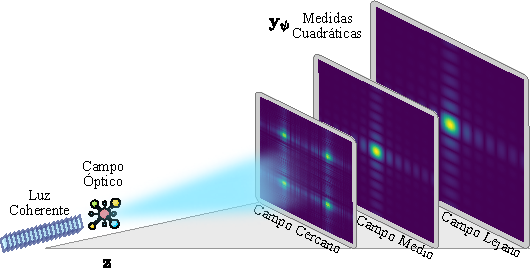
\includegraphics[width=0.9\linewidth]{images/marco_teórico/diffraction_no_coded.pdf}
    \label{fig:difraction_systems}
\end{figure}

Matemáticamente, la adquisición de medidas cuadráticas $\mathbf{y}_{\psi}\in\mathbb{R}^n$ en cada campo de difracción $\psi$ se puede modelar como 

\begin{equation}
    \mathbf{y}_{\psi}= \vert \mathbf{A}_\psi \mathbf{z} \vert^2,
    \label{eq:diffraction_base}
\end{equation}

donde $\vert \cdot \vert$ denota la magnitud, y $\mathbf{A}_\psi\in\mathbb{C}^{n \times n}$ es la matriz que modela el sistema de adquisición según cada campo de difracción. Particularmente, el objeto de interés contiene información de magnitud y fase $\mathbf{z}=\vert \mathbf{z}|\odot e^{j\mathrm{ang}(\mathbf{z})}$ con $j=\sqrt{-1}$, donde $\mathrm{ang}(\cdot)$ devuelve la fase de un vector complejo. La matriz $\mathbf{A}_\psi$ se define como

\begin{equation}
    \mathbf{A}_\psi = \left\{\begin{matrix}
 \mathbf{F}\mathbf{T}\mathbf{F}^\mathcal{H}    & \text{si } \psi=1\rightarrow \text{Campo cercano}\\ 
 \mathbf{F}^\mathcal{H}\mathbf{Q} &\text{si } \psi=2\rightarrow\text{ Campo medio} \\ 
 \mathbf{F}  &\text{si } \psi=3\rightarrow\text{Campo lejano}
\end{matrix}\right., \label{eq:matrix_a_no_coded}
\end{equation}

donde $\mathbf{F}\in\mathbb{C}^{n\times n}$ corresponde a la transformada discreta de Fourier, $\mathbf{Q}\in\mathbb{C}^{n\times n}$ y $\mathbf{T}\in\mathbb{C}^{n\times n}$ representan matrices que describen las funciones de transferencia usadas en óptica de Fourier \myfootcite{poon2014introduction} para modelar la difracción en el campo cercano y medio, respectivamente, dadas por
\begin{equation}
(\mathbf{Q})_{p,q}=e^{\frac{-jk_0}{2z}(p^2\delta_x^2+q^2\delta_y^2)},\label{eq:Qfuncion}
\end{equation}
\begin{equation}
(\mathbf{T})_{r,s}=e^{-jk_0z\sqrt{1-\frac{(r\delta_{kx})^2}{k_0^2}-\frac{(s\delta_{ky})^2}{k_0^2}}}.\label{eq:Tfuncion}
\end{equation}
Aquí, $k_0=2\pi/\lambda$ representa el número de onda, $[p,q]$ y $[r,s]$ son los índices discretos de las muestras en el dominio espacial y el dominio de Fourier, respectivamente. Los términos $\delta_x$ y $\delta_y$ son el periodo de muestreo en las coordenadas espaciales, y $\delta_{kx}$ y $\delta_{ky}$ son el periodo de muestreo en las coordenadas de las frecuencias. 

% Es importante resaltar que en este documento, la notación de variables $x, y$ y $z$ hace referencia a coordenadas cartesianas, mientras que $\mathbf{x}, \mathbf{y}$ y $\mathbf{z}$ en negrita se refieren al objeto, las medidas cuadráticas, y la estimación del objeto, respectivamente.


\section{PROBLEMA DE RECUPERACIÓN DE FASE}

La recuperación del campo óptico inicial $\mathbf{z}$ usando medidas cuadráticas es un problema inverso comúnmente denominado recuperación de fase. En general, el problema de recuperación de fase basado en \eqref{eq:diffraction_base} se puede definir como 

\begin{equation}
    \minimize_{\mathbf{z}\in\mathbb{C}^n}\Vert\mathbf{y}_{\psi} - \vert \mathbf{A}_{\psi}\mathbf{z} \vert\Vert_2^2, 
    \label{eq:phase_retrieval_problem}
\end{equation}

donde $\Vert \cdot\Vert_2$ es la norma euclidiana. Usualmente, se puede garantizar una recuperación que conserva un error de fase global \eqref{eq:phase_retrieval_problem} \myfootcite{eldar2014phase, gross2017improved, 9062527}, es decir que, $\hat{\mathbf{z}} = \hat{\mathbf{z}}e^{j\theta}$ con $\theta \in [0, 2\pi)$. En consecuencia, la distancia euclidiana entre la escena $\mathbf{z}$ y su estimación $\hat{\mathbf{z}}$ está dada por
\begin{equation}
    \mathrm{dist}(\mathbf{z}, \hat{\mathbf{z}}) = \min_{\theta \in [0, 2\pi)}\Vert \mathbf{z}e^{-j\theta} - \tilde{\mathbf{z}}\Vert_2.
\end{equation}

Adicionalmente, el problema inverso \eqref{eq:phase_retrieval_problem} se ha resuelto creando redundancia en el proceso de medición al incluir una máscara de fase, que permite la modulación del campo óptico, produciendo medidas cuadráticas codificadas según cada campo de difracción.

% Cabe señalar que, la información de fase en el plano Fourier es de suma importancia para garantizar la recuperación de la señal adquirida. La Figura \ref{fig:mescla_fases} ilustra un experimento desarrollado en \myfootcite{shechtman2015phase} donde se intercambia la información de fase de la transformada de Fourier de dos imágenes, posteriormente, se aplica la transformada de Fourier inversa a este intercambio. Aquí, se puede observar que en la imagen resultante predomina la información de las fases contrarias.

% \begin{figure}[!h]
%     \centering
%     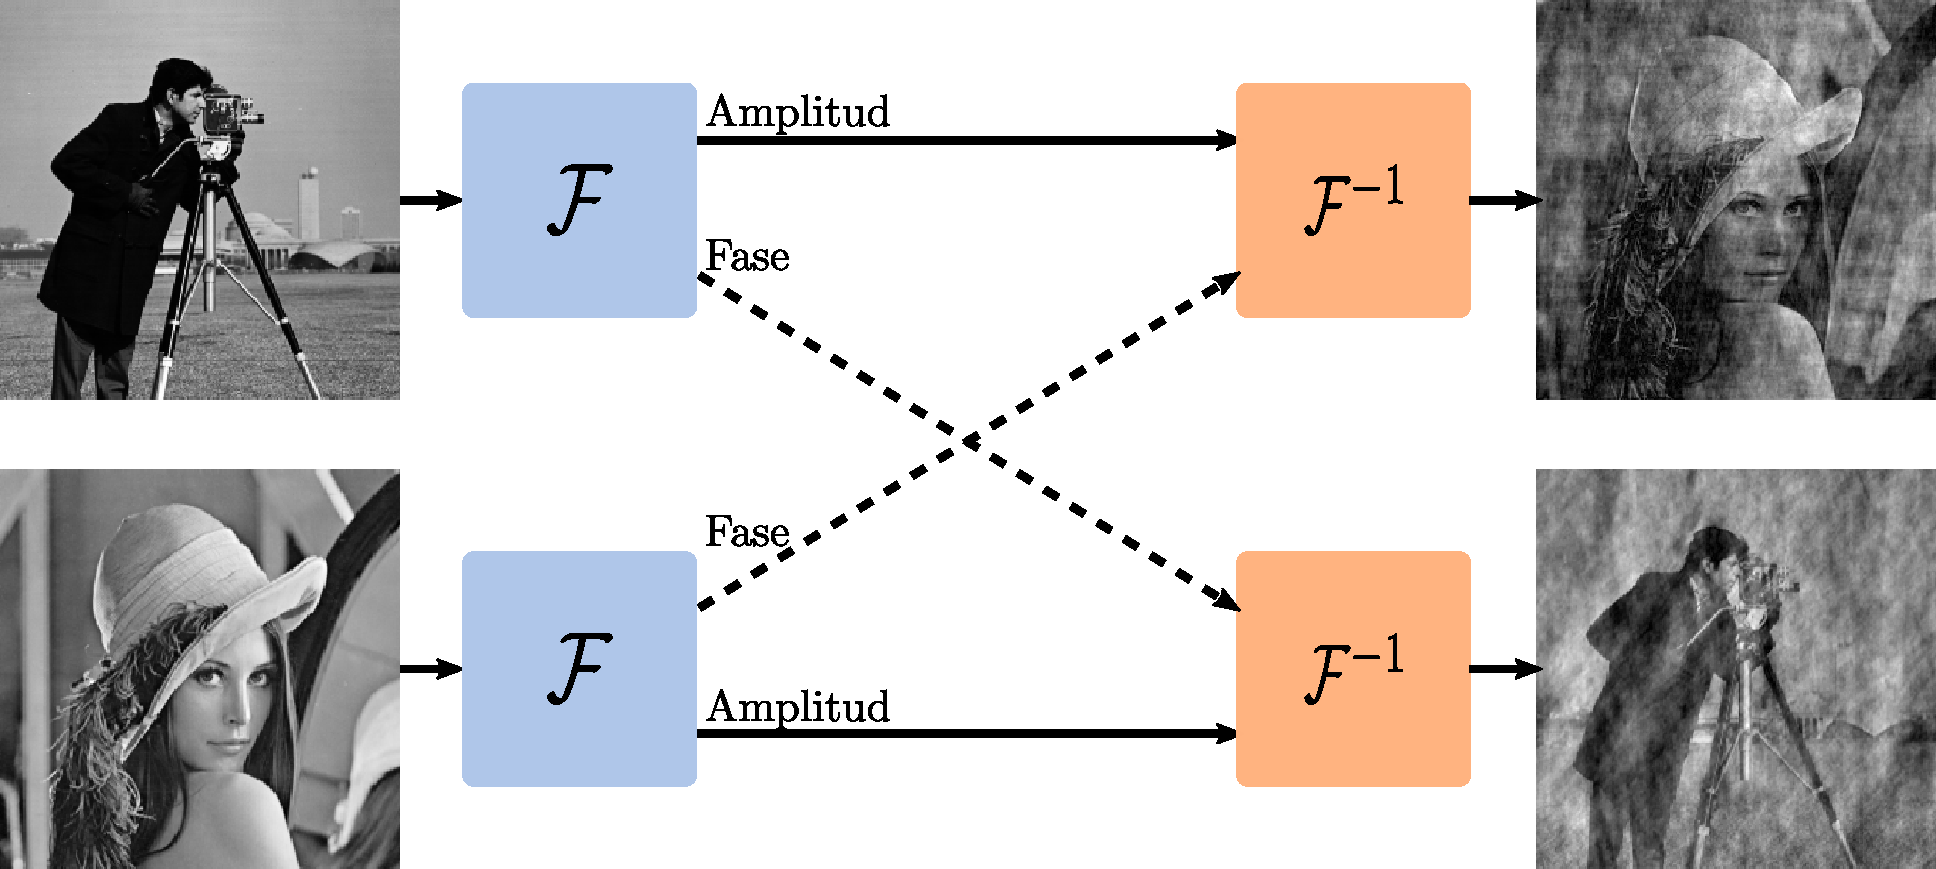
\includegraphics[width=0.9\linewidth]{images/marco_teórico/mescla_abs_fase.pdf}
%     \caption{\hspace{2mm}Experimento intercambiando la información de fase de la transformada de Fourier.}
%     \label{fig:mescla_fases}
% \end{figure}


% \pagebreak
\section{MEDIDAS CUADRÁTICAS CODIFICADAS}
Aquí, se describe el sistema de adquisición que capta medidas cuadráticas codificadas de un campo óptico a lo largo de cada campo de difracción. La Figura \ref{fig:coded_difraction_systems} ilustra el esquema de adquisición de medidas cuadráticas codificadas que incluye una máscara de codificación de fase $\mathbf{D}_\ell \in \mathbb{C}^{n\times n}$ para modular el campo óptico inicial. De hecho, al modificar la configuración espacial de la máscara de fase es posible adquirir múltiples proyecciones de la escena. De modo que, las proyecciones cuadráticas codificadas en cada campo de difracción para la $\ell$-ésima proyección está dada por 
\begin{equation}
    \mathbf{y}_{\ell, \psi} = \vert \mathbf{A}_{\ell, \psi}\mathbf{z} \vert, \ell=\{1,\dots,L\},
    \label{eq:phase_retrieval_problem}
\end{equation}

donde $\mathbf{A}_{\ell, \psi}\in\mathbb{C}^{n\times n}$ es la matriz que describe la $\ell$-ésima proyección según la propagación de cada campo de difracción $\psi$, siendo $L$ el número total de proyecciones. 
\begin{figure}[!h]
    \centering
    \caption{\hspace{2mm}Sistema óptico de difracción codificado.}
    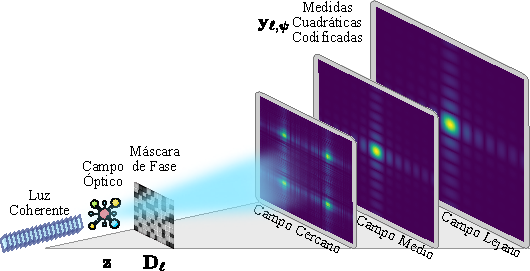
\includegraphics[width=0.9\linewidth]{images/marco_teórico/diffraction_coded.pdf}
    \label{fig:coded_difraction_systems}
\end{figure}

Específicamente, la matriz del sistema de adquisición $\mathbf{A}_{\ell, \psi}$ introduciendo una máscara de fase, se puede expresar como

\begin{equation}
    \mathbf{A}_{\ell,\psi}= \left\{\begin{matrix}
\mathbf{F}\mathbf{T}\mathbf{F}^\mathcal{H} \mathbf{D}_\ell  & \text{si } \psi=1\rightarrow \text{Campo cercano}\\ 
\mathbf{F}^\mathcal{H}\mathbf{Q}\mathbf{D}_\ell &\text{si } \psi=2\rightarrow\text{ Campo medio} \\ 
\mathbf{F}\mathbf{D}_\ell  &\text{si } \psi=3\rightarrow\text{Campo lejano}
\end{matrix}\right.. \label{eq:matrix_a}
\end{equation}
En general, las entradas aleatorias de la matriz  $\mathbf{D}_{\ell} = \mathrm{diag}(\mathbf{d})$ son $i.i.d$ copias de una variable aleatoria $d \in \mathbb{C}$ con $\mathbf{d} \in \{d\}^{n}$, donde $\mathrm{diag}(\cdot)$ devuelve una matriz diagonal cuadrada de un vector dado. Aquí, $d$ representa una modulación pasiva en la fase, por lo tanto, se impone que $d$ no aumenta la energía de la escena durante el proceso de modulación. Así que, se establece la Definición \ref{def:admissible} para garantizar la admisibilidad de la variable aleatoria.

\begin{definition}{(Variable aleatorias admisible). \myfootcite{9062527}} 
    Una variable aleatoria que cumple con $|d|\leq 1$, se considera admisible como elemento de modulación en fase.\label{def:admissible}
\end{definition}


Algunos ejemplos de variables aleatorias que satisfacen la Definición \ref{def:admissible} se listan en la Tabla \ref{tab:admi_examples}. Estas variables aleatorias como elementos de codificación han sido usados en \myfootcite{9062527} para resolver el problema de recuperación de fase.

\begin{table}[!h]
\centering
\caption{Ejemplos de codificaciones aleatórias admisibles según la Definición \ref{def:admissible}.}
\begin{tabular}{|c|c|}
\hline
\textbf{Elemento de codificación} & \textbf{Probabilidad}                     \\ \hline
$d \in \{0, 1\}$         & $\{ \frac{1}{2},  \frac{1}{2}\}$ \\ \hline
$d \in \{-1, 1\}$        & $\{ \frac{1}{2},  \frac{1}{2}\}$ \\ \hline
$d \in \{-1, 1, -j,  j\}$ & $\{ \frac{1}{4},  \frac{1}{4}, \frac{1}{4},  \frac{1}{4}\}$ \\ \hline
\end{tabular}
\label{tab:admi_examples}
\end{table}

% Cabe destacar que, en este trabajo de investigación se emplearon máscaras aleatorias con valores de $d \in \{-1, 1, -j,  j\}$, debido a sus características estadísticas \myfootcite{9062527}.

% \begin{equation}
%     \vert d \vert \leq M, \quad \mathbb{E}[d] = 0, \quad  \mathbb{E}[d^2] = 0, \quad  \mathbb{E}[\vert d \vert^4] = 2\mathbb{E}[\vert d \vert^2]^2,    
%     \label{eq:restricciones_mascara}
% \end{equation}

% donde $\mathbb{E}[\cdot]$ corresponde al valor esperado. Aquí, se busca que $M=1$ para que la codificación no incremente la potencia de las medidas cuadráticas.

\chapter{ALGORITMOS DE RECUPERACIÓN DE FASE}
En esta sección, se presentan los algoritmos comúnmente utilizados para recuperar el campó óptico inicial a partir de medidas cuadráticas codificadas. La literatura ha planteado diferentes algoritmos basados en formulaciones convexas y no convexas.

\section{FORMULACIONES CONVEXAS}

Este tipo de algoritmos relajan el problema recuperación de fase a un problema convexo equivalente.

\begin{itemize}
    \item \textbf{PhaseLift \myfootcite{candes2013phaselift}}:
    este algoritmo plantea el problema de recuperación de fase como una minimización de la traza de la siguiente forma
    \begin{equation}
        \begin{aligned}
            \minimize_{\mathbf{z} \in \mathbb{C}^{n}} \quad & \quad \mathrm{Traza}(\mathbf{z}\mathbf{z}^{\mathcal{H}}), \\
            \subjectto \quad & \quad \mathcal{A}(\mathbf{z}\mathbf{z}^{\mathcal{H}}) = \mathbf{b}, \\
             &\quad  \mathbf{z}\mathbf{z}^{\mathcal{H}} \succ 0,
        \end{aligned}
    \end{equation}
    
    donde $\mathcal{A}( \cdot ): \mathbb{R}^{n} \rightarrow \mathbb{R}^{m}$ es un operador lineal y $\mathrm{Traza}(\cdot)$ representa la traza de una matriz.
    
    \item \textbf{PhaseMax} \myfootcite{goldstein2018phasemax}:
    sea $\mathbf{\hat{z}} \in \mathbb{C}^{n}$ un vector aproximación de la señal original $\mathbf{z}$, de modo que, la señal reconstruida se obtiene solucionando el siguiente problema convexo
        
    \begin{equation}
        \begin{aligned}
            \maximize_{\mathbf{z}\in \mathbb{C}^n} \quad & \langle \mathbf{z}, \mathbf{\hat{z}} \rangle_{\mathbb{R}}, \\
            \subjectto \quad & \vert \langle \mathbf{a}_i,\mathbf{z} \rangle \vert \leq (\boldsymbol{\phi})_i,
        \end{aligned}
    \end{equation}
    donde $\langle \cdot, \cdot \rangle_{\mathbb{R}}$ denota la parte real del producto interno y $(\boldsymbol{\phi})_i = \sqrt{(\mathbf{y})_i}$
    
\end{itemize}

\section{FORMULACIONES NO CONVEXAS}
Las formulaciones no convexas requieren una estimación inicial de la escena o inicialización, además, calculan el gradiente siguiendo la diferenciación de Wirtinger.
\begin{itemize}
    \item \textbf{TRUNCATED WIRTINGER FLOW (TWF) \myfootcite{chen2017solving}:} este algoritmo se basa en el modelo de muestreo según un variables aleatorias que siguen una distribución de Poisson de la forma
    
    \begin{equation}
        (\mathbf{y})_i\sim \mathrm{Poisson}( \vert \langle \mathbf{a}_i,\mathbf{z}\rangle \vert^2 ), \quad i=1,\dots,m.
    \end{equation}
    
    TWF busca minimizar la máxima estimación de probabilidad 
    
    \begin{equation}
        \minimize_{z \in \mathbb{C}^{n}} - \sum_{i=1}^{m} \ell(\mathbf{z};\mathbf{y}_i),
    \end{equation}
    
    donde $\ell(\mathbf{z};\mathbf{y}_i) = { \mathbf{y}_i\log(|\mathbf{a}_i^H \mathbf{z}|^2) -|\mathbf{a}_i^H \mathbf{z}|^2 }$ con $(\cdot)^H$ el operador de conjugada transpuesta
    
    \item \textbf{TRUNCATED AMPLITUDE FLOW (TAF) \myfootcite{wang2017solving}:} este algoritmo adopta un criterio de mínimos cuadrados para recuperar $\mathbf{z}$ basado en las medidas sin fase $\mathbf{y}$ 
    
    \begin{equation}
        \minimize_{\mathbf{z} \in \mathbb{C}^{n}} \frac{1}{2m} \sum_{i=1}^{m} (\vert \langle \mathbf{a}_i,\mathbf{z}\rangle \vert - (\boldsymbol{\phi})_i)^2,
    \end{equation}
    
    Este algoritmo asume que las medidas $\mathbf{y}_i$ provienen de un sistema gaussiano de la forma $\mathbf{y}_i \sim \mathcal{N}(\vert \langle \mathbf{a}_i,\mathbf{z}\rangle \vert^2, 1)$
    
    \item \textbf{REWEIGHTED AMPLITUDE FLOW (RAF) \myfootcite{wang2018phase}:} este algoritmo sigue el criterio de maximizar la estimación de probabilidad de la forma
    
    \begin{equation}
        \minimize_{z \in \mathbb{C}^{n}} -\sum_{i=1}^{m} \ell(\mathbf{z};(\boldsymbol{\phi})_i/(\mathbf{y})_i),
    \end{equation}
    
    donde en el caso de un muestreo con ruido gaussiano basado en la amplitud $\ell(\mathbf{z};\mathbf{y}_i) = (\vert \langle \mathbf{a}_i,\mathbf{z}\rangle \vert - (\boldsymbol{\phi})_i)^2$ o basado en la intensidad  $\ell(\mathbf{z};(\mathbf{y})_i) = (\vert \langle \mathbf{a}_i,\mathbf{z}\rangle \vert^2 - (\mathbf{y})_i)^2$. Por otra parte, basado en un muestreo con distribución de Poisson, $\ell(\mathbf{z};(\mathbf{y})_i) = {(\mathbf{y})_i \log(|\mathbf{a}_i^H \mathbf{z}|^2) -|\mathbf{a}_i^H \mathbf{z}|^2 }$ 
\end{itemize}





\chapter{SISTEMAS DE CLASIFICACIÓN}

La clasificación ha sido una de las tareas computacionales más abordadas en el estado del arte. Específicamente, dentro de los algoritmos de clasificación tradicionales se encuentran las máquinas de soporte vectorial, K vecinos más cercanos \myfootcite{kim12012comparing} y los enfoques basados en redes neuronales \myfootcite{li2019deep,li2018deep, wang2019development}.
\section{MÁQUINAS DE SOPORTE VECTORIAL}
Las máquinas de soporte vectorial (SVM, por su sigla en inglés) \myfootcite{suthaharan2016support} permiten la clasificación binaria, donde cada punto $n$-dimensional $\mathbf{x}_i$ tiene asociada una etiqueta de clase $c_i \in \{1,-1\}$.

Suponiendo que los datos de ambas clases son separables linealmente, este método propone separar los datos usando el hiperplano $\mathbf{w}\mathbf{x}_i + b = 0$. En la Figura \ref{fig:svm}, se muestra una representación de una SVM en $\mathbb{R}^2$

\begin{equation}
    \begin{split}
        \mathbf{w}\mathbf{x}_i + b &\geq 1 \quad si \quad c_i=1, \\
        \mathbf{w}\mathbf{x}_i + b &\leq 1 \quad si \quad c_i=-1.
    \end{split}
\end{equation}

Cabe resaltar que, para todos los elementos del conjunto de datos se cumple que

\begin{equation}
    c_i(\mathbf{w}\mathbf{x}_i + b) \geq 1, \quad i=1,\dots, m
\end{equation}

\begin{figure}[H]
    \centering
    \caption{\hspace{2mm}Representación de una SVM en $\mathbb{R}^2$. La recta $\mathbf{wx} -b = 0$ en rojo representa el plano óptimo que soluciona el problema de optimización \eqref{eq:problema_optimización_svm}.}
    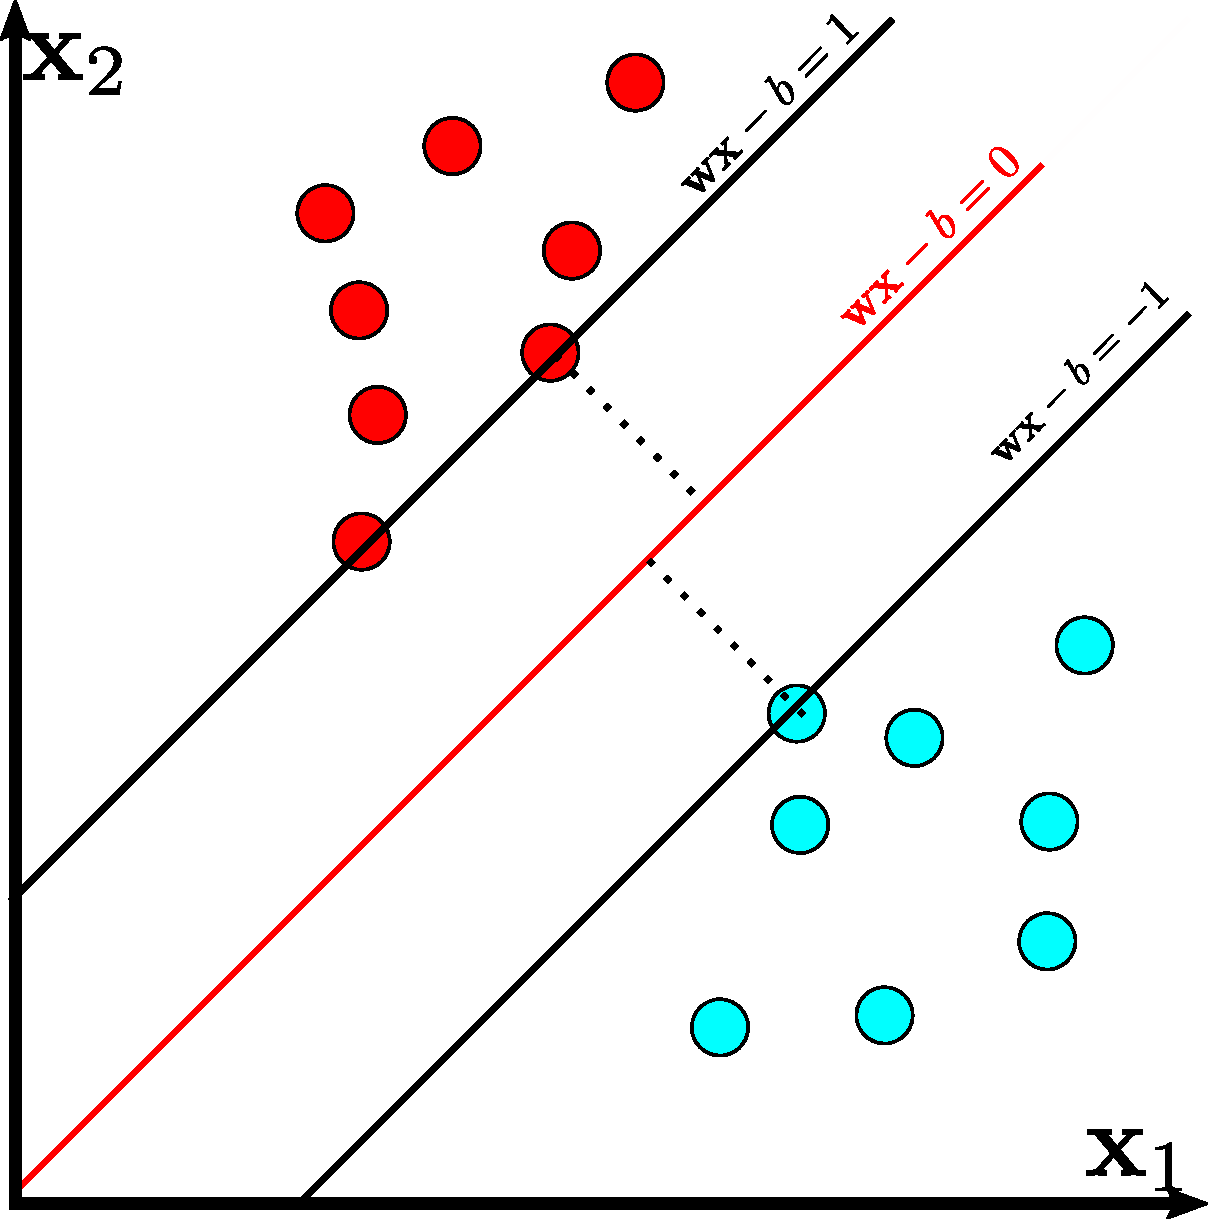
\includegraphics[width=0.4\linewidth]{images/marco_teórico/svm.pdf}
    \label{fig:svm}
\end{figure}

El problema de optimización se plantea de la siguiente forma

\begin{equation}
    \begin{aligned}
        \minimize_{\mathbf{w}} & \quad \Vert \mathbf{w} \Vert, \\
        \subjectto_{\quad i=1,\dots, m} & \quad c_i(\mathbf{w}\mathbf{x}_i + b) \geq 1.
    \end{aligned}
    \label{eq:problema_optimización_svm}
\end{equation}

Usualmente, no es posible separar los datos linealmente, por esta razón, se puede incluir una función no lineal $ \phi$ que transforme los datos a un conjunto de características donde las clases sean separables linealmente. El problema de optimización para una SVM usando un kernel $\phi$ se formula como

\begin{equation}
    \begin{aligned}
        \minimize_{\mathbf{w}} & \quad \Vert \mathbf{w} \Vert, \\
        \subjectto_{\quad i=1,\dots, m} & \quad c_i(\mathbf{w}\phi(\mathbf{x}_i) + b) \geq 1.
    \end{aligned}
\end{equation}


\section{K VECINOS MÁS CERCANOS}

K vecinos más cercanos (KNN, por sus siglas en inglés) propone que un conjunto $D = \{(\mathbf{x}_i, {c}_i)\}_1^n$, siendo $\mathbf{x}_i$ el vector de características e $\mathbf{c}_i$ la clase correspondiente. Para un nuevo vector a clasificar $\mathbf{\hat{x}}$, el algoritmo KNN encuentra los $K$ puntos más cercanos del dataset. La Figura \ref{fig:knn} muestra una representación de la clasificación de dos nuevas muestras en $\mathbb{R}^2$ con $K = 5$. Tradicionalmente, se emplea la distancia euclidiana 

\begin{equation}
    d(\mathbf{x}_p,\mathbf{x}_q) = \Vert \mathbf{x}_p-\mathbf{x}_q \Vert_2
    \label{eq:distancia_euclidiana}
\end{equation}

\begin{figure}[H]
    \centering
    \caption{\hspace{2mm}Representación de KNN en $\mathbb{R}^2$ con $K = 5$.}
    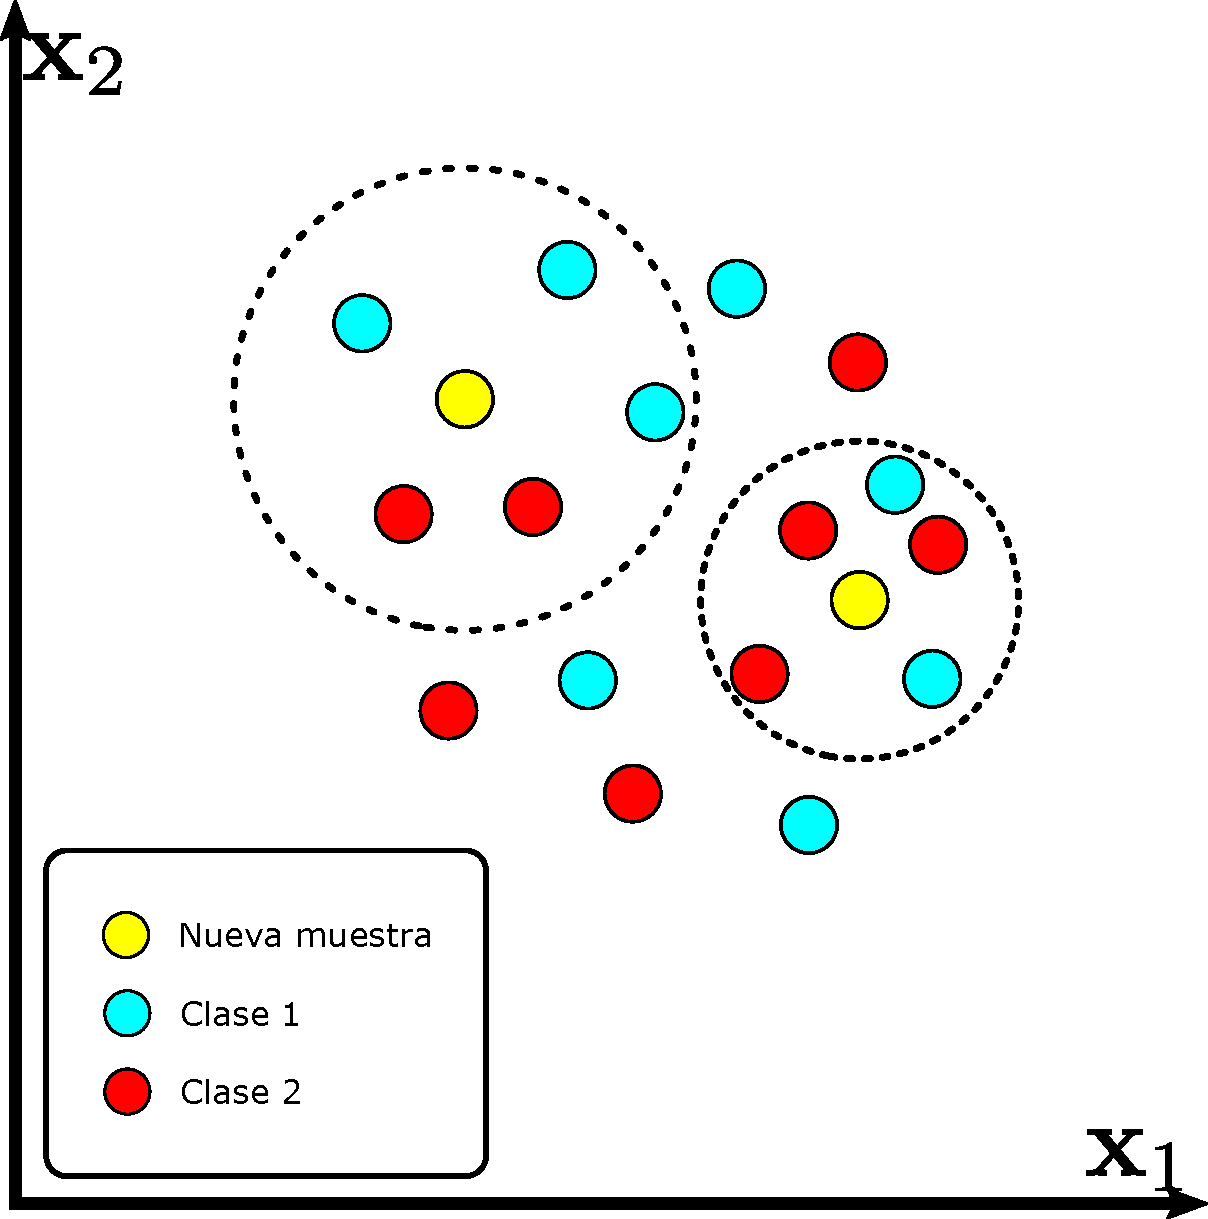
\includegraphics[width=0.4\linewidth]{images/marco_teórico/knn.pdf}
    \label{fig:knn}
\end{figure}

Posteriormente, con base en las clases de los $K$ puntos encontrados, de tal forma que, $C \subset D$ y $\vert C \vert = K$, se cuantifica la cantidad de veces que aparece cada clase y se clasifica la nueva muestra $\mathbf{\hat{x}}$ con la clase que más veces aparezca de la forma

\begin{equation}
    \mathrm{clase}(\mathbf{\hat{x}}) =  \argmax_{\hat{c}} \bigg\{ \sum_{\hat{c} \in C} \delta(C,\hat{c})\bigg\},
\end{equation}

donde $\delta(\cdot,\cdot)$ corresponde a la función delta de Kronecker, dada por

\begin{equation}
    \delta(a,b) = \begin{cases}
        1, \quad a = b \\
        0, \quad a \neq b
    \end{cases}
\end{equation}
\section{REDES NEURONALES}

Los enfoques de aprendizaje profundo han generado un gran progreso en problemas muy complejos en los últimos años
\myfootcite{he2016deep,li2019deep,li2018deep, wang2019development,vaswani2017attention}. El aprendizaje profundo busca encontrar una función $f: \mathbb{R}^{d_1} \rightarrow \mathbb{R}^{d_2}$ que relacione un dato de entrada con una respectiva salida. La función $f$ comúnmente se denomina arquitectura de red neuronal profunda, puesto que, consiste en la concatenación de múltiples capas compuestas por unidades mínimas llamadas neuronas. Cada neurona realiza una combinación lineal entre las entradas, posteriormente, se emplea una función no lineal en la salida. Las salidas de cada neurona en una capa funcionan como entrada de las neuronas ubicadas en la siguiente capa, por lo tanto, se construye una arquitectura de red neuronal profunda \myfootcite{fan2019selective}. En la Figura \ref{fig:nn}, se muestra una arquitectura de una arquitectura de red neuronal $f: \mathbb{R}^{d_1} \rightarrow \mathbb{R}^{d_2}$.

\begin{figure}[H]
    \centering
    \caption{\hspace{2mm}Esquema de una arquitectura de red neuronal $f: \mathbb{R}^{d_1} \rightarrow \mathbb{R}^{d_2}$.}
    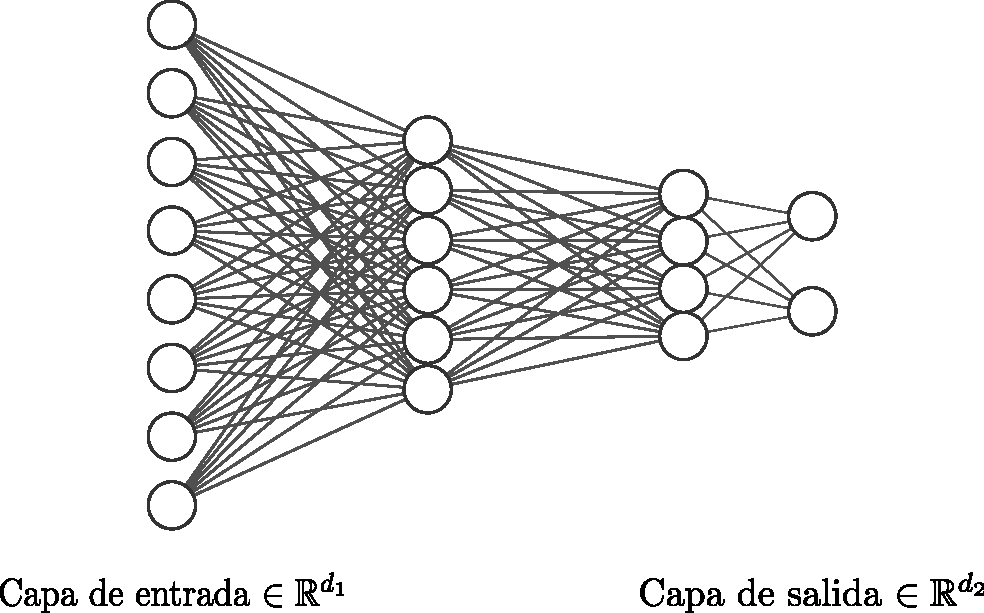
\includegraphics[width=0.6\linewidth]{images/marco_teórico/nn.pdf}
    \label{fig:nn}
\end{figure}

Por otra parte, el modelo matemático de una red neuronal estándar se puede definir como
\begin{equation}
    \footnotesize 
    \big\{f_\theta(\mathbf{x}) = \sigma_{J}(\mathbf{W}_{J}\sigma_{J-1}(\mathbf{W}_{J-1} (\dots \sigma_2(\mathbf{W}_2\sigma_1(\mathbf{W}_1\mathbf{x} + \mathbf{b}_1) + \mathbf{b}_2))  + \mathbf{b}_{J-1})  + \mathbf{b}_J) \quad \vert \quad\theta = \{\mathbf{W}_{j}, \mathbf{b}_{j}\}  \big\},
    \label{eq:red_neuronal}
\end{equation}

donde $1 \leq j \leq J$ representa cada una de las capas que compone la red neuronal, $\sigma_j$ corresponde a una función no lineal en dicha capa, $\mathbf{W}_j$ es la matriz de pesos y $\mathbf{b}_j$ es el bias de la capa. Con el fin de entrenar los pesos $\theta$ bajo un enfoque de aprendizaje supervisado, se requiere de un conjunto de entrenamiento $\{(\mathbf{x}_k, c_k) \}_{k=1}^{N}$ y una función de costo $\mathcal{L}( c_k,  f_\theta(\mathbf{x}_k))$ para plantear el problema de optimización 

\begin{equation}
    \minimize_\theta \frac{1}{N}\sum_{k=1}^{N} \mathcal{L}( {c}_k,  f_\theta(\mathbf{x}_k))
    \label{eq:optimización_nn}
\end{equation}
\section{CLASIFICACIÓN DE IMÁGENES USANDO REDES NEURONALES ÓPTICAS}


Recientemente, se han publicado avances en el campo de redes neuronales implementadas físicamente haciendo uso de propiedades ópticas. En este tipo de redes, se destaca la velocidad de la inferencia, puesto que, esta se realiza de manera óptica, es decir, la velocidad de cálculo está limitada por la velocidad de la luz en el medio y no requiere de una fuente de energía activa para realizar los cálculos. Específicamente, \myfootcite{lin2018all} implementa las capas de una red neuronal haciendo uso de materiales difractivos, realizando la modulación de la luz en fase y aprovechando la propagación del campo óptico para realizar tareas de clasificación.


\begin{figure}[!h]
    \centering
    \caption{Implementación de redes neuronales ópticas implementadas ópticamente mediante elementos ópticos difractivos.}
    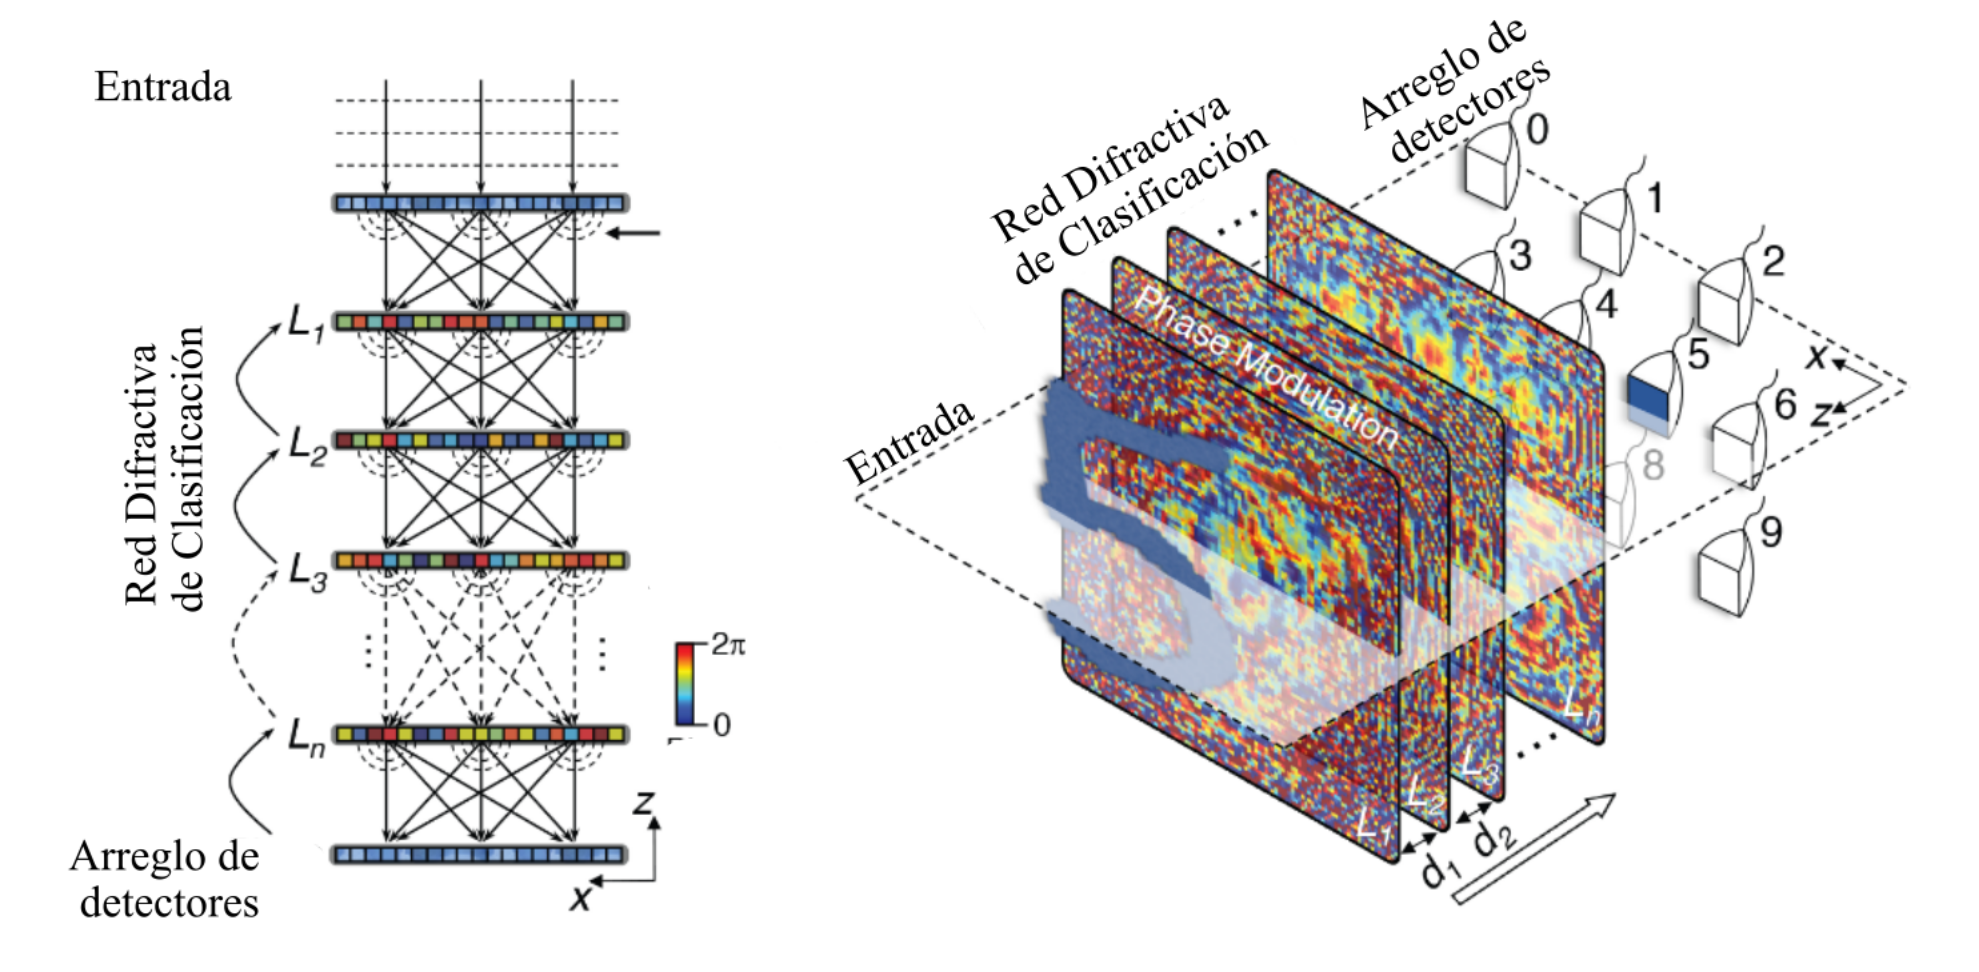
\includegraphics[width = 1\linewidth]{images/marco_teórico/diffractive_networks.png}
    \caption*{Modificado de: \textit{All-optical machine learning using diffractive deep neural networks, 2018.}}
    \label{fig:optical_networks}
\end{figure}

\section{CLASIFICACIÓN USANDO MEDIDAS CUADRÁTICAS}
En el campo de tomografía computarizada \myfootcite{douarre2020value} e imágenes de un solo píxel \myfootcite{bacca2020coupled}, se han propuesto sistemas de clasificación que usan únicamente medidas obtenidas a través de sistemas lineales de adquisición, esto debido al enfoque basado en el aprendizaje profundo en el que la arquitectura incluye una capa con el sistema óptico de adquisición. Asimismo, este enfoque ha sido estudiado en holografía \myfootcite{kim2018deep} y cristalografía de rayos-x \myfootcite{ziletti2018insightful}, donde las medidas obtenidas son difícilmente reconocidas por el ojo humano. 

Sin embargo, estos enfoques de clasificación tradicionales no han sido abordados en imágenes de medidas cuadráticas codificadas, por lo tanto, este trabajo propone el desarrollo de un algoritmo de clasificación de objetos usando medidas cuadráticas codificadas bajo un enfoque de aprendizaje profundo. 




